% ============================================================
% Capítulo I (Volumen II) — Teoría elástica de la luz
% Traducción de "Théorie mathématique de la lumière II" (1892)
% Original: §§1-11, páginas impresas 1-18
% ============================================================
\chapter{Teoría elástica de la luz}
\label{cap:vol2-elastica}

\section{Movimiento del éter}

\noindent\textbf{1. Movimiento del éter.} — Esta teoría atribuye los
fenómenos luminosos a las vibraciones de un medio elástico, el éter,
difundido en todo el espacio, incluso en el vacío.

Sea una molécula de éter que, en el estado de equilibrio, ocupa la
posición $M$: a consecuencia de la vibración, vendrá a ocupar una posición
tal como $M'$. El vector $MM'$ se llama el desplazamiento de la molécula.
Si $x,y,z$ designan las coordenadas del punto $M$, y $x+\xi,\,y+\eta,\,z+\zeta$
las del punto $M'$, las proyecciones del desplazamiento sobre los tres ejes
de coordenadas serán $\xi,\eta,\zeta$.

Las componentes de la velocidad de la molécula según los mismos ejes serán
\[
\frac{d\xi}{dt},\qquad \frac{d\eta}{dt},\qquad \frac{d\zeta}{dt},
\]
y las componentes de la aceleración
\[
\frac{d^2\xi}{dt^2},\qquad \frac{d^2\eta}{dt^2},\qquad \frac{d^2\zeta}{dt^2}.
\]

Consideremos un pequeño paralelepípedo rectángulo $ABCDEFGH$
(figura~\ref{fig:vol2-cap1-1}), cuyas aristas sean paralelas a los ejes y tengan
respectivamente por longitud $dx,dy,dz$: el volumen de este paralelepípedo
será $d\tau=dx\,dy\,dz$. Durante la vibración, este paralelepípedo se
desplaza y toma una posición tal como $A'B'C'D'E'F'G'H'$; se convierte en
un paralelepípedo curvilíneo, que puede asimilarse, despreciando
infinitésimos de segundo orden, a un paralelepípedo rectilíneo, pero
oblicuo.

Pongamos
\[
\alpha_1=\frac{d\xi}{dx},\qquad \alpha_2=\frac{d\eta}{dy},\qquad \alpha_3=\frac{d\zeta}{dz};
\]
\[
\beta_1=\frac{d\eta}{dz}+\frac{d\zeta}{dy};\qquad
\beta_2=\frac{d\zeta}{dx}+\frac{d\xi}{dz};\qquad
\beta_3=\frac{d\xi}{dy}+\frac{d\eta}{dx}.
\]
Se demuestra (véase el \emph{Cours d'élasticité}, p.~7) que las longitudes
de las aristas del paralelepípedo se convierten en
\[
dx(1+\alpha_1)\qquad dy(1+\alpha_2)\qquad dz(1+\alpha_3).
\]
Por esta razón $\alpha_1,\alpha_2,\alpha_3$ se llaman las dilataciones
lineales.

Los tres ángulos del triedro $A$, que eran los tres iguales a $\pi/2$, se
convierten respectivamente, en el triedro $A'$, en
\[
\frac{\pi}{2}+\beta_1,\qquad \frac{\pi}{2}+\beta_2,\qquad \frac{\pi}{2}+\beta_3.
\]
$\beta_1,\beta_2,\beta_3$ se llaman las dilataciones angulares.

En cuanto a la diagonal $AH$, se convierte en $A'H'$, y su longitud es
función de las seis dilataciones.

\begin{figure}[ht]
\centering
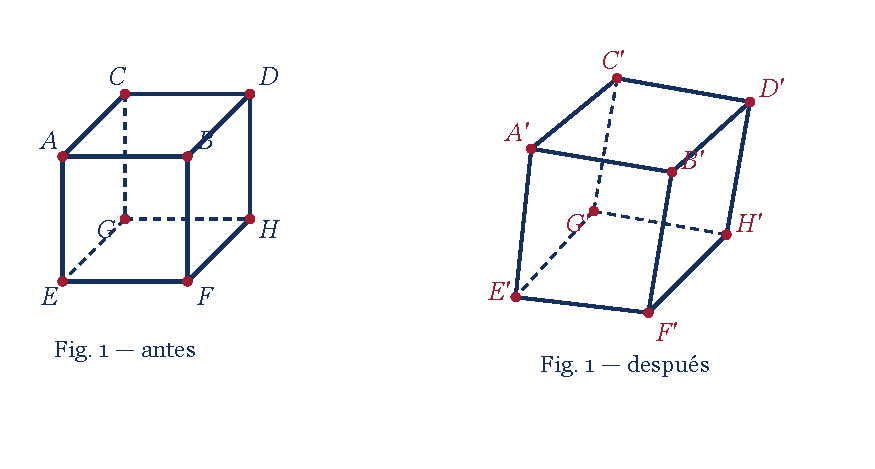
\includegraphics[width=0.85\textwidth]{figuras/pdf/cap01-fig1.pdf}
\caption{El paralelepípedo $ABCDEFGH$ antes y después de la vibración,
convertido en el paralelepípedo oblicuo $A'B'C'D'E'F'G'H'$.}
\label{fig:vol2-cap1-1}
\end{figure}

\section{Fuerza viva del éter}

\noindent\textbf{2. Fuerza viva del éter.} — Sea $\mathrm{T}$ la fuerza
viva o energía cinética del éter.\footnote{A diferencia del Volumen~I,
donde «fuerza viva» designa $\sum mv^2$, el doble de la energía cinética,
aquí Poincaré identifica expresamente la fuerza viva con la energía
cinética $\sum mv^2/2$, como muestra la expresión de $\mathrm{T}$ que
sigue. Conservamos el término tal como él lo usa.~(N.~del T.)} Tenemos, como expresión del cuadrado de
la velocidad,
\[
V^2=\left(\frac{d\xi}{dt}\right)^2+\left(\frac{d\eta}{dt}\right)^2+\left(\frac{d\zeta}{dt}\right)^2.
\]
La masa del pequeño paralelepípedo es $\rho\,d\tau$, siendo $\rho$ la
densidad del éter. Por consiguiente
\[
\mathrm{T}=\sum\frac{mv^2}{2}
=\frac{1}{2}\int\rho\,d\tau\left[\left(\frac{d\xi}{dt}\right)^2
+\left(\frac{d\eta}{dt}\right)^2+\left(\frac{d\zeta}{dt}\right)^2\right].
\]

\section{Energía potencial del éter}

\noindent\textbf{3. Energía potencial del éter.} — Se ha demostrado, en el
\emph{Cours d'élasticité}, p.~43, §26 y siguientes, que la energía
potencial tenía una expresión de la forma
\[
\mathrm{U}=\int \mathrm{W}\,d\tau,
\]
siendo $\mathrm{W}$ un polinomio de segundo grado respecto de las nueve
derivadas parciales de primer orden de $\xi,\eta,\zeta$.

Si suponemos que el medio es isótropo y que en el estado de equilibrio la
presión es nula, obtendremos
\[
\mathrm{W}=\mu\left(\alpha_1^2+\alpha_2^2+\alpha_3^2
+\frac{\beta_1^2}{2}+\frac{\beta_2^2}{2}+\frac{\beta_3^2}{2}\right)+\lambda\frac{\theta^2}{2}.
\]
$\lambda$ y $\mu$ son los coeficientes de Lamé; $\theta$ está definido por
la igualdad
\[
\theta=\alpha_1+\alpha_2+\alpha_3=\frac{d\xi}{dx}+\frac{d\eta}{dy}+\frac{d\zeta}{dz}.
\]
Se demuestra que un elemento de volumen $d\tau$ se convierte, tras la
deformación, en
\[
d\tau(1+\theta),
\]
de donde el nombre de dilatación cúbica dado a $\theta$.

\section{Valor de las fuerzas}

\noindent\textbf{4. Valor de las fuerzas.} — Retomemos el paralelepípedo
$ABCDEFGH$, y consideremos en particular la cara $ACEG$ perpendicular a
$Ox$ (figura~\ref{fig:vol2-cap1-2}): el área de esta cara es igual a
$dy\,dz$. Llamaremos $\mathrm{P}_{xx},\mathrm{P}_{xy},\mathrm{P}_{xz}$ a
las componentes según los ejes de la presión que se ejerce sobre esta cara
por unidad de área, y convendremos en considerar las tensiones como
positivas, y las presiones como negativas.

Las componentes de la presión que se ejerce sobre la cara $ACEG$ serán,
pues,
\[
\mathrm{P}_{xx}\,dy\,dz,\qquad \mathrm{P}_{xy}\,dy\,dz,\qquad \mathrm{P}_{xz}\,dy\,dz.
\]
Tendremos del mismo modo, para la cara $ABEF$ perpendicular a $Oy$,
\[
\mathrm{P}_{yx}\,dx\,dz,\qquad \mathrm{P}_{yy}\,dx\,dz,\qquad \mathrm{P}_{yz}\,dx\,dz,
\]
y para la cara $EFGH$ perpendicular a $Oz$,
\[
\mathrm{P}_{zx}\,dx\,dy,\qquad \mathrm{P}_{zy}\,dx\,dy,\qquad \mathrm{P}_{zz}\,dx\,dy.
\]
Según la teoría de la elasticidad,
\[
\mathrm{P}_{xy}=\mathrm{P}_{yx}\qquad \mathrm{P}_{yz}=\mathrm{P}_{zy}\qquad \mathrm{P}_{zx}=\mathrm{P}_{xz}
\]
y
\[
\mathrm{P}_{xx}=\frac{d\mathrm{W}}{d\alpha_1}=\lambda\theta\frac{d\theta}{d\alpha_1}+2\mu\alpha_1
=\lambda\theta+2\mu\alpha_1=\lambda\theta+2\mu\frac{d\xi}{dx}
\]
\[
\mathrm{P}_{yy}=\lambda\theta+2\mu\frac{d\eta}{dy}
\]
\[
\mathrm{P}_{zz}=\lambda\theta+2\mu\frac{d\zeta}{dz}
\]
\[
\mathrm{P}_{xy}=\mu\beta_3=\mu\left(\frac{d\xi}{dy}+\frac{d\eta}{dx}\right)
\]

\begin{figure}[ht]
\centering
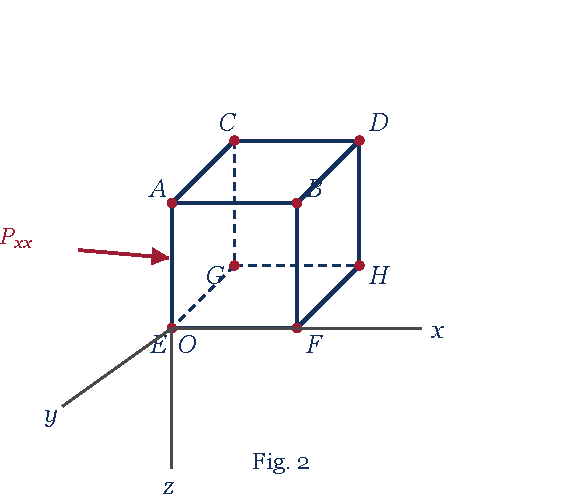
\includegraphics[width=0.7\textwidth]{figuras/pdf/cap01-fig2.pdf}
\caption{La cara $ACEG$, perpendicular a $Ox$, sobre la que se ejerce la
presión $\mathrm{P}_{xx}$.}
\label{fig:vol2-cap1-2}
\end{figure}

\section{Ecuaciones del movimiento}

\noindent\textbf{5. Ecuaciones del movimiento.} — Escribiendo que la
fuerza de inercia equilibra a las fuerzas que actúan sobre el elemento
$d\tau$, obtendremos las ecuaciones del movimiento:\footnote{En la
expresión que sigue, el original imprime $dy\,dx$ como último factor del
segundo renglón y $d\mathrm{P}_{xz}/dx$ en el tercero, y escribe
$d^2\zeta/dt^2$ en el primer miembro de la ecuación~(1); son
erratas evidentes por $dz\,dx$ (área de la cara perpendicular a $Oy$),
$d\mathrm{P}_{xz}/dz$ y $d^2\xi/dt^2$, como muestran el
primer miembro de la expresión desarrollada y la ecuación que se obtiene a
continuación por sustitución.~(N.~del T.)}
\[
\begin{aligned}
\rho\,dx\,dy\,dz\cdot\frac{d^2\xi}{dt^2}
={}&-\mathrm{P}_{xx}\,dy\,dz+\left(\mathrm{P}_{xx}+\frac{d\mathrm{P}_{xx}}{dx}dx\right)dy\,dz\\
&-\mathrm{P}_{xy}\,dz\,dx+\left(\mathrm{P}_{xy}+\frac{d\mathrm{P}_{xy}}{dy}dy\right)dz\,dx\\
&-\mathrm{P}_{xz}\,dx\,dy+\left(\mathrm{P}_{xz}+\frac{d\mathrm{P}_{xz}}{dz}dz\right)dx\,dy
\end{aligned}
\]
o bien
\begin{equation}
\rho\frac{d^2\xi}{dt^2}=\frac{d\mathrm{P}_{xx}}{dx}+\frac{d\mathrm{P}_{xy}}{dy}+\frac{d\mathrm{P}_{xz}}{dz}
\tag{1}
\end{equation}
y otras dos que se obtendrían por permutación. Por otra parte,
\[
\mathrm{P}_{xx}=\mu\frac{d\xi}{dx}+\mu\frac{d\xi}{dx}+\lambda\theta,\qquad
\mathrm{P}_{xy}=\mu\frac{d\xi}{dy}+\mu\frac{d\eta}{dx},\qquad
\mathrm{P}_{xz}=\mu\frac{d\xi}{dz}+\mu\frac{d\zeta}{dx}.
\]
Sustituyendo estas expresiones en la ecuación (1), resulta
\[
\rho\frac{d^2\xi}{dt^2}=\mu\Delta\xi+\mu\frac{d\theta}{dx}+\lambda\frac{d\theta}{dx}.
\]
Las ecuaciones del movimiento serán, pues,
\begin{equation}
\begin{gathered}
\rho\frac{d^2\xi}{dt^2}=\mu\Delta\xi+(\lambda+\mu)\frac{d\theta}{dx},\\[3pt]
\rho\frac{d^2\eta}{dt^2}=\mu\Delta\eta+(\lambda+\mu)\frac{d\theta}{dy},\\[3pt]
\rho\frac{d^2\zeta}{dt^2}=\mu\Delta\zeta+(\lambda+\mu)\frac{d\theta}{dz}.
\end{gathered}
\tag{I}
\end{equation}

\section{Ondas planas}
\label{sec:vol2-cap1-ondas-planas-1}

\noindent\textbf{6. Ondas planas.} — En el caso de las ondas planas,
$\xi$ y $\eta$ no dependen más que de $z$ y de $t$. Por consiguiente,
\[
\Delta\xi=\frac{d^2\xi}{dz^2}\qquad \Delta\eta=\frac{d^2\eta}{dz^2}\qquad
\theta=\frac{d\zeta}{dz}\qquad \Delta\zeta=\frac{d^2\zeta}{dz^2}.
\]
Las derivadas tomadas respecto de $x$ y de $y$ son nulas, y las ecuaciones
del movimiento se reducen a
\[
\rho\frac{d^2\xi}{dt^2}=\mu\frac{d^2\xi}{dz^2}\qquad
\rho\frac{d^2\eta}{dt^2}=\mu\frac{d^2\eta}{dz^2}\qquad
\rho\frac{d^2\zeta}{dt^2}=\mu\frac{d^2\zeta}{dz^2}+(\lambda+\mu)\frac{d^2\zeta}{dz^2}
=(\lambda+2\mu)\frac{d^2\zeta}{dz^2}.
\]
Estas ecuaciones son las de las cuerdas vibrantes.

Supongamos que el desplazamiento sea paralelo a $Ox$:
\[
\eta=\zeta=0 \qquad \xi\neq 0.
\]
El plano de onda es paralelo al plano $xy$. La vibración es transversal.
Solo queda, pues, la ecuación
\[
\rho\frac{d^2\xi}{dt^2}=\mu\frac{d^2\xi}{dz^2}.
\]
Esta ecuación tiene por integral
\[
\xi=f\left(z+t\sqrt{\frac{\mu}{\rho}}\right)+f_1\left(z-t\sqrt{\frac{\mu}{\rho}}\right),
\]
siendo $f$ y $f_1$ funciones arbitrarias. Esta onda se propaga con la
velocidad $\sqrt{\mu/\rho}$.

Habríamos obtenido un resultado enteramente análogo suponiendo el
desplazamiento paralelo a $Oy$.

Si el desplazamiento es paralelo a $Oz$, subsiste únicamente la ecuación
\[
\rho\frac{d^2\zeta}{dt^2}=(\lambda+2\mu)\frac{d^2\zeta}{dz^2}.
\]
La integral
\[
\zeta=f\left(z+t\sqrt{\frac{\lambda+2\mu}{\rho}}\right)+f_1\left(z-t\sqrt{\frac{\lambda+2\mu}{\rho}}\right)
\]
representa una vibración longitudinal, puesto que el desplazamiento es
perpendicular al plano de onda, y la velocidad de propagación es
$\sqrt{(\lambda+2\mu)/\rho}$.

La experiencia nos enseña que las vibraciones luminosas son transversales.
En efecto, en los diversos fenómenos de reflexión o de refracción, se
recupera toda la fuerza viva del rayo incidente en los rayos de vibraciones
transversales. Si existieran rayos de vibraciones longitudinales, estos
absorberían una parte de esta fuerza viva.

Admitiremos, pues, que no existe vibración longitudinal en el rayo
luminoso, y por consiguiente que
\[
\lambda+2\mu=0.
\]

\section{Intensidad luminosa. Definición experimental}

\noindent\textbf{7. Intensidad luminosa. Definición experimental.} — Para
poder comparar con la experiencia las consecuencias de las ecuaciones, es
indispensable definir bien la cantidad que se mide en las experiencias, es
decir, la intensidad luminosa.

Es necesario incluso dar de esta intensidad dos definiciones, una
experimental, y la otra teórica; pues queremos comparar la teoría con la
experiencia, y para que esta comparación sea posible, hay que definir bien
los dos términos.

Experimentalmente, la intensidad se mide con ayuda de tres clases de
fenómenos: $1.^{\text{o}}$ los efectos fisiológicos; $2.^{\text{o}}$ los
efectos químicos (fotográficos); $3.^{\text{o}}$ los efectos caloríficos de
la luz. A cada una de estas clases de fenómenos corresponde una definición
de la intensidad. No es evidente \emph{a priori} que estas tres
definiciones sean equivalentes, y de hecho no lo son en absoluto. Sabemos,
por ejemplo, que la intensidad de la acción química de un rayo varía con su
color. Cuando se trata de comparar dos rayos homogéneos del mismo color, es
posible que el efecto fisiológico sea proporcional al efecto químico, y
así parece ocurrir en el caso de una onda plana; pero en los casos más
delicados, como en las experiencias recientes del señor Otto Wiener, solo
es posible un modo de evaluación, el que está fundado en la fotografía.

Somos, sin embargo, libres de adoptar una de estas definiciones y de
examinar sus consecuencias.

Convendremos, pues, en decir que dos luces tienen igual intensidad cuando
producen en el mismo tiempo la misma acción sobre una placa fotográfica;
que una luz tiene una intensidad mayor o menor que otra según que, en el
mismo tiempo, produzca sobre la placa sensible una acción mayor o menor
que esa otra.

Esta definición es puramente experimental.

\section{Definición teórica}

\noindent\textbf{8. Definición teórica.} — Desde el punto de vista
teórico, se ha considerado a menudo la intensidad como proporcional a la
fuerza viva media o energía cinética del éter.

Esta fuerza viva del éter, para el elemento de volumen $d\tau$, es igual a
\[
\rho\,d\tau\cdot\frac{v^2}{2},
\]
es decir, por unidad de masa, $v^2/2$.

Supongamos, por ejemplo, que la vibración sea rectilínea y tomemos como
eje de las $x$ la dirección de vibración en el punto considerado; entonces
\[
\eta=\zeta=0 \qquad v=\frac{d\xi}{dt};
\]
la fuerza viva será
\[
\frac{1}{2}\left(\frac{d\xi}{dt}\right)^2,
\]
y la intensidad será proporcional al valor medio de esta expresión.

Siendo el movimiento periódico, podemos poner
\[
\xi=\mathrm{A}\sin 2\pi\frac{t}{\mathrm{T}},
\]
eligiendo como origen del tiempo el instante en que $\xi=0$; $\mathrm{T}$
es el período; $\xi$ tiene por máximo $\mathrm{A}$ en valor absoluto;
$\mathrm{A}$ es la amplitud.
\[
\frac{d\xi}{dt}=\mathrm{A}\frac{2\pi}{\mathrm{T}}\cos 2\pi\frac{t}{\mathrm{T}}.
\]
La intensidad será, pues, proporcional a\footnote{El original da como
valor de esta integral $(\mathrm{A}^2/2)(4\pi^2/\mathrm{T}^2)$,
olvidando el factor $\frac12$ que proviene del valor medio de
$\cos^2 2\pi t/\mathrm{T}$ sobre un período. La omisión no afecta la
conclusión, que solo concierne a la proporcionalidad con
$\mathrm{A}^2$.~(N.~del T.)}
\[
\frac{1}{\mathrm{T}}\int_0^{\mathrm{T}}\frac{\mathrm{A}^2}{2}\frac{4\pi^2}{\mathrm{T}^2}
\cos^2 2\pi\frac{t}{\mathrm{T}}\,dt=\frac{1}{2}\cdot\frac{\mathrm{A}^2}{2}\frac{4\pi^2}{\mathrm{T}^2}.
\]
Es, pues, proporcional al cuadrado de la amplitud $\mathrm{A}$.

No es en absoluto evidente que así definamos la misma cosa que con la
definición experimental. Estamos tan autorizados a suponer que la acción
fotográfica es proporcional, no a la energía cinética media, sino a la
energía potencial o a la energía total media.

\noindent\textbf{9.} Estas diversas definiciones de la intensidad,
equivalentes en ciertos casos, como vamos a verlo, corresponden a maneras
distintas de concebir el mecanismo de la acción fotográfica.

Consideremos, en efecto, las moléculas de éter que, en su posición de
equilibrio, ocupan una esfera infinitamente pequeña $O$. Cuando el éter
entre en vibración, el centro de gravedad de la esfera oscilará de un lado
y otro de $O$, y al mismo tiempo la esfera se deformará: tomará una forma
asimilable a la de un elipsoide $O'$ (figura~\ref{fig:vol2-cap1-3}); los
ejes de este elipsoide ejecutarán también una serie de oscilaciones.

¿Depende la intensidad de la amplitud de las oscilaciones de $O$, o está
relacionada con la amplitud de las oscilaciones de los ejes del elipsoide?
No lo sabemos.

Si admitimos que la intensidad es proporcional a la fuerza viva media,
como las componentes de la velocidad son $d\xi/dt,d\eta/dt,d\zeta/dt$, la
intensidad dependerá de la variación de $\xi,\eta,\zeta$ con el tiempo, es
decir, del desplazamiento del punto $O$. Admitamos, al contrario, que la
intensidad es proporcional a la energía potencial media $\int \mathrm{W}\,d\tau$;
$\mathrm{W}$ depende de las dilataciones $\alpha$ y $\beta$; o bien aún de
los ejes del elipsoide (cf. \emph{Théorie de l'Élasticité}, p.~9); la
intensidad dependería entonces de la amplitud de las deformaciones de la
esfera, es decir, de las variaciones periódicas que experimenta la
distancia de dos moléculas, variaciones que son función de las $\alpha$ y
de las $\beta$.

Ignoramos la naturaleza de las acciones químicas de las que son sede las
placas fotográficas. Sin duda los átomos materiales correspondientes
experimentan el mismo desplazamiento, y podría uno sentirse tentado a
razonar así:

Supongamos que el desplazamiento del punto $O$ sea considerable, y las
deformaciones del elipsoide muy pequeñas. Nuestra esfera estará sometida
únicamente a un movimiento de traslación; la distancia de dos moléculas de
éter permanecerá invariable durante la vibración, y lo mismo ocurrirá con
la distancia de dos átomos materiales, puesto que hemos supuesto que el
desplazamiento del éter es el mismo que el de la materia ponderable. En
esta hipótesis se comprende difícilmente la disociación de la molécula
química. No podría, pues, haber acción química, por grande que fuera el
desplazamiento del punto $O$, cuando el elipsoide no se deformara. Se
concluiría, pues, que la intensidad depende de las variaciones de las
$\alpha$ y de las $\beta$, y no de las de $\xi,\eta,\zeta$.

Pero esta manera de ver no se impone.

Nada impide suponer que el desplazamiento del éter y el del átomo material
sean solo proporcionales, variando el coeficiente de proporcionalidad de un
átomo a otro, y se llegaría a una conclusión inversa.

En el primer orden de ideas, la intensidad sería proporcional a la energía
potencial media; en el segundo caso, a la fuerza viva media.

Pero, repitámoslo, ninguna de estas hipótesis se impone necesariamente.

Por lo demás, en la mayoría de los casos, y son justamente los únicos que,
hasta estos últimos años, hemos conseguido realizar en la práctica, las dos
definiciones son equivalentes; esto ocurre cuando se trata de ondas
planas.

\begin{figure}[ht]
\centering
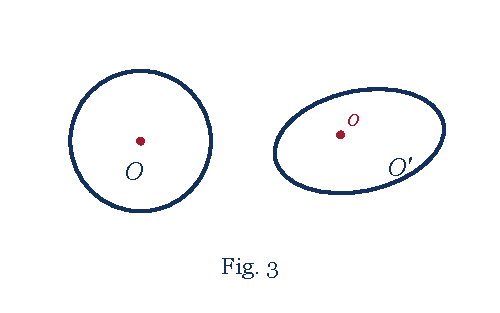
\includegraphics[width=0.6\textwidth]{figuras/pdf/cap01-fig3.pdf}
\caption{La esfera $O$, en su posición de equilibrio, se deforma en el
elipsoide $O'$; $o$ es el centro de gravedad desplazado.}
\label{fig:vol2-cap1-3}
\end{figure}

\section{Ondas planas}
\label{sec:vol2-cap1-ondas-planas-2}

\noindent\textbf{10. Ondas planas.} — Tomemos el plano de la onda como plano $xy$.

$\xi,\eta,\zeta$ serán funciones de $z$ y de $t$ solamente. Si la
vibración es transversal, tendremos
\[
\zeta=0
\]
\[
\xi=f\left(z-t\sqrt{\tfrac{\mu}{\rho}}\right)+f_1\left(z+t\sqrt{\tfrac{\mu}{\rho}}\right)
\]
\[
\eta=\varphi\left(z-t\sqrt{\tfrac{\mu}{\rho}}\right)+\varphi_1\left(z+t\sqrt{\tfrac{\mu}{\rho}}\right).
\]
El primer término en cada una de estas expresiones representa una
perturbación que se propaga hacia los $z$ positivos. El segundo, una
perturbación que se propaga hacia los $z$ negativos. Supondremos que
existe una sola de estas perturbaciones, sin lo cual habría interferencia
y nuestros razonamientos ya no serían válidos.

Pondremos, pues,
\[
\xi=f\left(z-t\sqrt{\frac{\mu}{\rho}}\right),\qquad
\eta=\varphi\left(z-t\sqrt{\frac{\mu}{\rho}}\right),
\]
por consiguiente
\[
\frac{d\xi}{dz}=f'\qquad \frac{d\eta}{dz}=\varphi'
\]
\[
\frac{d\xi}{dt}=-f'\sqrt{\frac{\mu}{\rho}}=-\frac{d\xi}{dz}\sqrt{\frac{\mu}{\rho}}
\qquad
\frac{d\eta}{dt}=-\varphi'\sqrt{\frac{\mu}{\rho}}=-\frac{d\eta}{dz}\sqrt{\frac{\mu}{\rho}}.
\]

La intensidad definida por la energía cinética media es proporcional al
valor medio de
\[
\left(\frac{d\xi}{dt}\right)^2+\left(\frac{d\eta}{dt}\right)^2.
\]

Calculemos ahora la energía potencial $\mathrm{W}$, considerando la
energía localizada en un elemento de volumen $d\tau$ y refiriéndola a la
unidad de volumen:
\[
\mathrm{W}=\mu\left(\alpha_1^2+\alpha_2^2+\alpha_3^2+\frac{\beta_1^2}{2}
+\frac{\beta_2^2}{2}+\frac{\beta_3^2}{2}\right)+\lambda\frac{\theta^2}{2}.
\]
En el caso actual todas las derivadas tomadas respecto de $x$ y de $y$ son
nulas, además $\zeta=0$, así como todas sus derivadas. Por tanto,
\[
\alpha_1=\alpha_2=\alpha_3=0\qquad \theta=0\qquad \beta_3=0
\]
\[
\beta_1=\frac{d\eta}{dz}\qquad \beta_2=\frac{d\xi}{dz}
\]
\[
\mathrm{W}=\frac{\mu}{2}\left[\left(\frac{d\eta}{dz}\right)^2+\left(\frac{d\xi}{dz}\right)^2\right].
\]

Puesto que $d\eta/dt$ y $d\xi/dt$ son proporcionales a $d\eta/dz$ y
$d\xi/dz$, las intensidades dadas por las dos definiciones son, pues,
proporcionales entre sí.

\section{Otras formas de las ecuaciones del movimiento}

\noindent\textbf{11. Otras formas de las ecuaciones del movimiento.} —
Hemos encontrado, para representar el movimiento
del éter, las ecuaciones
\[
\rho\frac{d^2\xi}{dt^2}=\mu\Delta\xi+(\lambda+\mu)\frac{d\theta}{dx}.
\]

Para que las vibraciones longitudinales tengan una velocidad
constantemente nula, es necesario que
\[
\lambda+2\mu=0.
\]
Introduzcamos esta condición, y las ecuaciones se convierten en
\begin{equation}
\begin{gathered}
\rho\frac{d^2\xi}{dt^2}=\mu\left(\Delta\xi-\frac{d\theta}{dx}\right)\\[3pt]
\rho\frac{d^2\eta}{dt^2}=\mu\left(\Delta\eta-\frac{d\theta}{dy}\right)\\[3pt]
\rho\frac{d^2\zeta}{dt^2}=\mu\left(\Delta\zeta-\frac{d\theta}{dz}\right)
\end{gathered}
\tag{II}
\end{equation}
Si las vibraciones son transversales, tenemos, en el origen del tiempo,
\[
\theta=0\qquad \frac{d\theta}{dt}=0,
\]
y $\theta$ permanece nulo en una época cualquiera. En efecto,
diferenciemos las ecuaciones (II)\footnote{El original dice aquí
«les équations (2)»; se trata evidentemente de las ecuaciones~(II) que
acaban de escribirse.~(N.~del T.)} respecto de $x,y,z$ y sumemos; resulta
\[
\rho\frac{d^2\theta}{dt^2}=\mu(\Delta\theta-\Delta\theta)=0
\]
\[
\frac{d^2\theta}{dt^2}=0
\]
\[
\theta=\mathrm{A}+\mathrm{B}t.
\]
$\mathrm{A}$ y $\mathrm{B}$ son independientes del tiempo. Si, pues, para
$t=0$ tenemos
\[
\theta=0\qquad\text{y}\qquad \frac{d\theta}{dt}=0,
\]
$\theta$ es idénticamente nulo. Es ordinariamente lo que se supone, y las
ecuaciones del movimiento toman entonces la forma
\begin{equation}
\rho\frac{d^2\xi}{dt^2}=\mu\Delta\xi\qquad
\rho\frac{d^2\eta}{dt^2}=\mu\Delta\eta\qquad
\rho\frac{d^2\zeta}{dt^2}=\mu\Delta\zeta
\tag{III}
\end{equation}
Pongamos
\begin{equation}
\frac{1}{\mu}\frac{du}{dt}=\frac{d\zeta}{dy}-\frac{d\eta}{dz}.
\tag{IV}
\end{equation}
Esta relación no define $u$ más que salvo una constante; supondremos que
para $t=0$ se tiene
\[
\xi=\eta=0\qquad \frac{du}{dt}=0.
\]
Pondremos del mismo modo:\footnote{El original repite aquí la misma
etiqueta «(IV)» para este segundo par de ecuaciones, en vez de darles un
número nuevo: las tres relaciones que definen $u$, $v$ y $w$, deducidas
unas de otras por la permutación cíclica de $\xi,\eta,\zeta$, forman un
solo sistema~(IV), y así lo cita Poincaré al final del párrafo («la
primera de las ecuaciones~(IV)» es la que define~$u$). Conservamos su
numeración. Además, en la segunda de estas relaciones el original imprime
$d\zeta/dy$ en lugar de $d\xi/dy$; es una errata
evidente, como muestran la permutación cíclica y la expresión de
$d^2w/dy\,dt$ que se forma a continuación.~(N.~del T.)}
\begin{equation}
\begin{gathered}
\frac{1}{\mu}\frac{dv}{dt}=\frac{d\xi}{dz}-\frac{d\zeta}{dx}\\[3pt]
\frac{1}{\mu}\frac{dw}{dt}=\frac{d\eta}{dx}-\frac{d\xi}{dy}.
\end{gathered}
\tag{IV}
\end{equation}

Formemos la expresión
\[
\frac{d^2w}{dy\,dt}-\frac{d^2v}{dz\,dt}.
\]
\[
\frac{d^2w}{dy\,dt}=\mu\left(\frac{d^2\eta}{dx\,dy}-\frac{d^2\xi}{dy^2}\right)
\]
\[
-\frac{d^2v}{dz\,dt}=\mu\left(\frac{d^2\zeta}{dx\,dz}-\frac{d^2\xi}{dz^2}\right)
\]
\[
0=\mu\left(\frac{d^2\xi}{dx^2}-\frac{d^2\xi}{dx^2}\right).
\]
Sumemos miembro a miembro:
\[
\frac{d^2w}{dy\,dt}-\frac{d^2v}{dz\,dt}=\mu\left(\frac{d\theta}{dx}-\Delta\xi\right).
\]
Por consiguiente,
\[
\rho\frac{d^2\xi}{dt^2}=-\left(\frac{d^2w}{dy\,dt}-\frac{d^2v}{dz\,dt}\right).
\]
Integremos respecto de $t$:
\[
\rho\frac{d\xi}{dt}=-\left(\frac{dw}{dy}-\frac{dv}{dz}\right).
\]
Según la hipótesis que hemos hecho sobre las condiciones iniciales, la
constante de integración es nula.

Las ecuaciones del movimiento podrán, pues, ponerse bajo la forma
\begin{equation}
\begin{gathered}
\rho\frac{d\xi}{dt}=-\left(\frac{dw}{dy}-\frac{dv}{dz}\right)\\[3pt]
\rho\frac{d\eta}{dt}=-\left(\frac{du}{dz}-\frac{dw}{dx}\right)\\[3pt]
\rho\frac{d\zeta}{dt}=-\left(\frac{dv}{dx}-\frac{du}{dy}\right)
\end{gathered}
\tag{V}
\end{equation}

Bajo esta forma, se ve que no cambian cuando se permuta
\[
\xi,\eta,\zeta \text{ en } u,v,w;\qquad u,v,w \text{ en } -\xi,-\eta,-\zeta;
\qquad \rho \text{ en } \frac{1}{\mu}\text{ y } \mu \text{ en } \frac{1}{\rho}.
\]
Efectuemos, en efecto, esta permutación sobre la primera de las
ecuaciones, la que define $u$: resulta
\[
-\rho\frac{d\xi}{dt}=\frac{dw}{dy}-\frac{dv}{dz},
\]
y efectuándola sobre la primera de las ecuaciones (V),\footnote{El
original dice aquí «la première des équations (IV)»; es una errata por
(V): la primera de las ecuaciones~(IV) es justamente la que acaba de
transformarse, y es la primera de las~(V),
$\rho\,d\xi/dt=-(dw/dy-dv/dz)$, la que, con
$\xi\to u$, $v\to-\eta$, $w\to-\zeta$, $\rho\to 1/\mu$, da la relación
siguiente.~(N.~del T.)} obtendremos
\[
\frac{1}{\mu}\frac{du}{dt}=\frac{d\zeta}{dy}-\frac{d\eta}{dz}.
\]

Estas ecuaciones no dan más que una primera aproximación en los medios
transparentes ordinarios, a causa de los fenómenos de dispersión: presentan
una mayor exactitud en el vacío.
